\documentclass{../notes}
\title{Pullback: Buying support/Shorting resistance}
\begin{document}
\maketitle

\section{Setup}
\begin{itemize}
  \item Presence of a good impulse setting up further continuation.
  \item Market is not overextended.
  \item Market is not on the third (or later) trend leg.
  \item Absence of momentum divergence.
  \item Absence of buying or selling climax.
  \item Pullbacks show generally lower activity (bar range) and volume than the trend legs.
  \item Absence of strong countertrend momentum
\end{itemize}

\section{Trigger}
Buy against support level near bottom or selling short against resistance on top of pullback
\subsection{Support/resistance usually slopes in pullbacks}
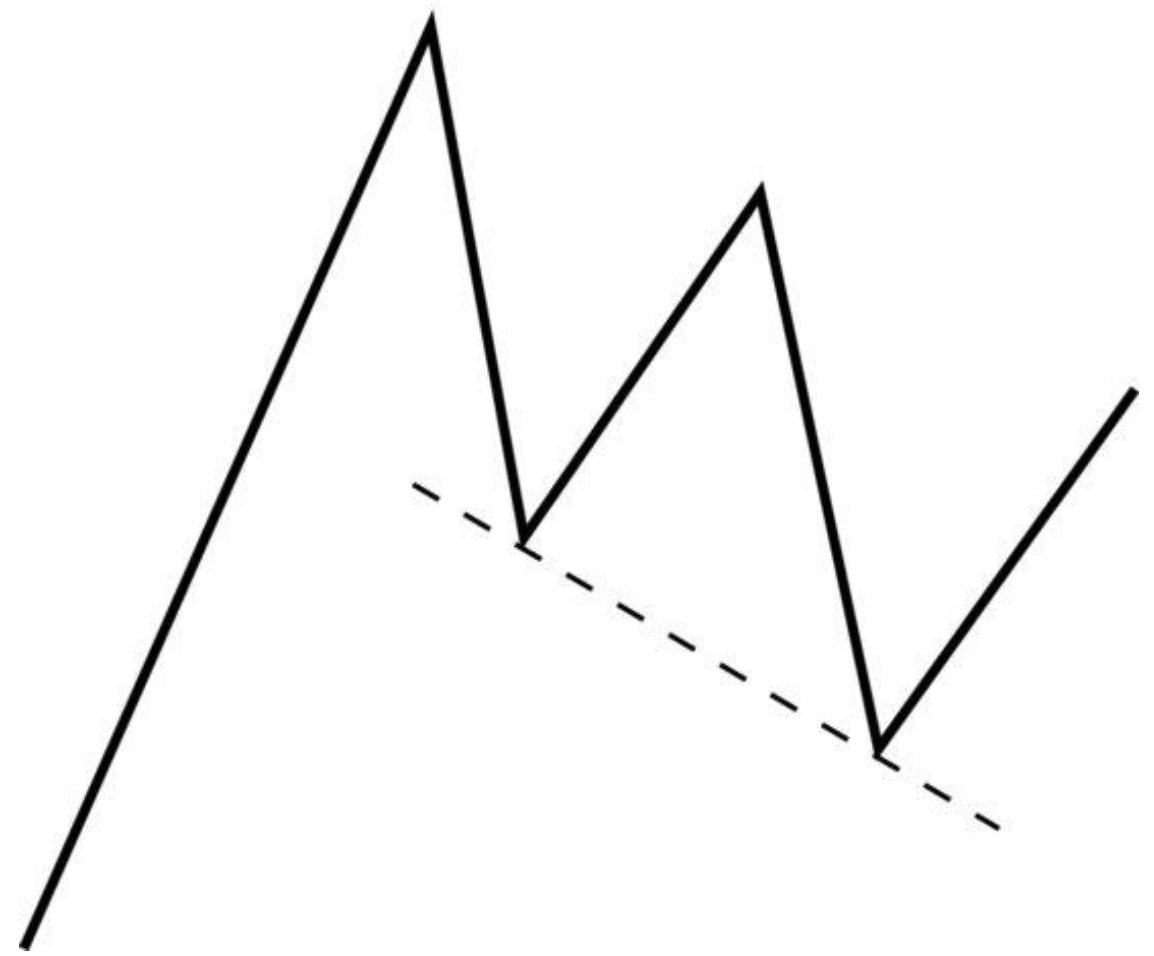
\includegraphics[width=0.4\linewidth]{pullback-slope-down}
\begin{itemize}
  \item Does not make sense to exit a trade that is within the loping level
\end{itemize}

\subsection{Trigger 1: Lower time frame climax}
\begin{enumerate}
  \item Draw a parallel trend line pullback
  \begin{enumerate}
    \item First draw a standard linear trendline for lower timeframe between higher lows in an uptrend (demand line) or lower highs for downtrend (supply line)
    \item Create a parallel line to the opposite side of the trend (attach to pivot highs in uptrend) BETWEEN the initial two anchor points for standard trend line. Also must not cut through prices between the two initial anchor points
  \end{enumerate}
  \item Price drops past support, but immediately recover within a few bars (lower time-frame climax), but should be clear from default timeframe
\end{enumerate}
Note this is not a buy-and-forget entry. Needs experience and to pay attention because most likely exhausiton below support happens in a single bar.

\subsection{Trigger 2: Bottom of support}
\begin{enumerate}
  \item See a bounce back in pullback. Draw horizontal line at peak.
  \item Buy when when price reaches support again.
  \item Must not be buying into 3rd or more test of support (ie, only buying after one bounce). If support is tested for third or more times, reduce exposure.
\end{enumerate}
\section{Stop}
\begin{itemize}
  \item Crucial to have a stop loss.
  \item Recommend to set one further away from pattern and add in a few cents beyond obvious levels
  \item Can change stops dramatically a few bars into a trade
  \item Can use a time stop
\end{itemize}
\section{Profit Target}
\begin{itemize}
  \item Most conservative profit target is previous pivot high of the setup leg
  \item Good exit plan allows taking partial profits and holding onto portion of position for further trend legs
  \item Can use MMO profit targets, but recommend to take majority or all profits even though trade has not quite reached the target
\end{itemize}
\section{Comments}









\end{document}
